
\chapter{SCCD}
\label{chap:sccd}

In this chapter, I will talk about SCCD. In the MSDL laboratory, they use SCCD to simulate Statechart. After a presentation of my project in July, they suggested me to try their simulator and compare it to the Ciprian simulator. It is possible to find more explanation about SCCD on the Master's thesis published by Glenn De Jonghe\cite{sccd} and on the Master's thesis published by Joeri Exelmans\cite{sccd2}.

\section{Short description}

SCCD\footnote{signified StateChart and Class Diagram} is an open source simulator and code generator of Statechart developed by the MSDL laboratory. SCCD need some specificities in models, a class Diagram and a StateChart attached on each classes. It also use some special semantics to instantiate classes with an object manager.

Because a state machine is a statechart\footnote{Statechart is an extension of state machine, invented by David Harel}, for the rest of this chapter we can consider that our models verify the SCCD's specificities.


\section{Transformer}

As we see before, the project has been written to have a ability to change the simulator. However, the model need to be written in scxml standard to be interpreted by SCCD. So the first things that I have to do is a transformer in XSLT. XSLT is a language for transforming XML documents into other XML documents.
~\\

After some research on the internet I found only one transformer written by apache on Github\cite{apache}. The last commit of this project was in 2009, so we can assume that the project is abandoned. I had tried to use it but it didn't work. For this reason I have created a new transformer, but I used some part of this project.
~\\

My transformer have the ability to transform a xmi file as a scxml file. However, model given by my professor had some specificities so I take care to adapt to its.

For example, when there is a script in ABCD language and the script is <<send eventA to itsPinger>> the translation in the state machine is <<raise eventA to itsPinger>>. Then I use the fact that our project always have a \textit{SUS} class which contains all other classes, so in the scxml model the \textit{SUS} class start all other classes.

\section{Utilization}

\subsection{SCCD debugger}

In my project I want to visualize states of all state machine. To do that, I need some informations of the status of the model. SCCD don't permit this type of utilization, but the SCCD debugger written by Simon Van Mierlo can do it.
~\\

However, during my internship this debugger wasn't finished. The debugger can create only one class because the object manager doesn't work.
~\\

To prove that my scxml model created automatically will work when the debugger will be finished, I tried to do a prove of contest. %I use my scxml model created by my transformer automatically in SCCD and I verify the running.

\subsection{SCCD}

To do this prove of contest, I achieve some tests on the pure SCCD. I use the last version of SCCD published in the beginning of august.


I quickly realize that my model had infinite loop. These loops are explain because in the model there is some state which have transition on itself, and this transitions are always verify. In the Ciprian simulator it was not a problem because the user has to choose the next transition and so he was the condition. To fix this problem I add on these transitions a timer of 1s.

The figure \ref{fig:sccd_resume} resume the work done to execute xmi model with SCCD. You can also see on the figure \ref{fig:sccd} the result of the Ping-Pong example on SCCD. As it was expected there is an event which is send from ping to pong and then from pong to ping.
\begin{figure}[h]
  \centering
  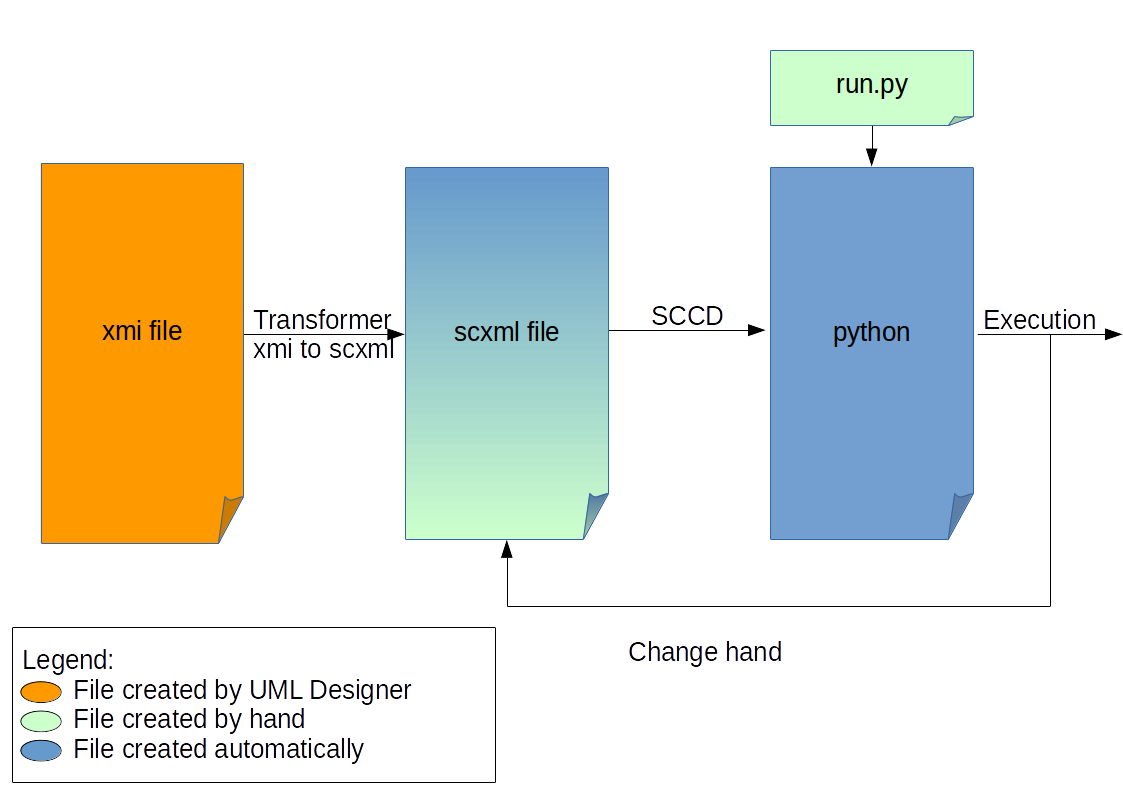
\includegraphics[width=\linewidth]{scxml}
  \caption{Resume}
  \label{fig:sccd_resume}
\end{figure}

\begin{figure}[h]
  \centering
  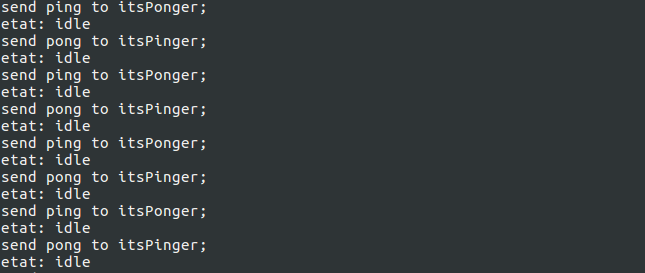
\includegraphics[width=\linewidth]{sccd}
  \caption{pingpong simulation on SCCD}
  \label{fig:sccd}
\end{figure}


%%% Local Variables:
%%% mode: latex
%%% TeX-master: "../rapport_de_base"
%%% End:
